% Groxel: voxel worlds with glued faces, traversed by permuting the stepping state.
%
% The bodies of the tables and the data of the plot are written by experiments/figures.py from
% the results in experiments/results/, and reproduce.sh at the top of the repository regenerates
% them and builds this file.
\documentclass[10pt,a4paper]{article}
\usepackage[margin=2.6cm]{geometry}
\usepackage[T1]{fontenc}
\usepackage[utf8]{inputenc}
\usepackage{microtype}
\usepackage{amsmath,amssymb,amsthm}
\usepackage{booktabs}
\usepackage{graphicx}
\usepackage{tikz}
\usetikzlibrary{arrows.meta,positioning,matrix}
\usepackage{pgfplots}
\pgfplotsset{compat=1.17}
\usepackage[hidelinks]{hyperref}
\usepackage[capitalise]{cleveref}

\newtheorem{proposition}{Proposition}
% Reads a generated table body. \input is not expandable, and a rule may not follow it.
\makeatletter\let\tablebody\@@input\makeatother
\newcommand{\code}[1]{\texttt{#1}}
\newcommand{\tmax}{t_{\max}}
\newcommand{\tdelta}{t_{\Delta}}

\definecolor{s1}{HTML}{2A78D6}
\definecolor{s2}{HTML}{EB6834}
\definecolor{s3}{HTML}{1BAF7A}
\definecolor{s4}{HTML}{EDA100}
\definecolor{s5}{HTML}{E87BA4}

\title{Groxel: voxel worlds with glued faces,\\traversed by permuting the stepping state}
\author{Keston Aquino-Michaels\\ No Way Labs\\ {\small\url{https://github.com/no-way-labs/groxel}}}
\date{November 2026}

\begin{document}
\maketitle

\begin{abstract}
A groxel world is a set of voxel rooms in which a rectangle of voxel faces can be glued to
another by one of the 48 symmetries of the cube and an integer shift. We describe an engine in
which that gluing is the only primitive: rays, flood-filled light, sprites and walking bodies all
move by crossing faces. A ray crosses a gluing by permuting its Amanatides--Woo stepping state,
and no part of the state is recalculated. In a space glued to itself on every face, 220{,}000 rays
that cross up to 1{,}000 gluings report the same voxel, face, step count and distance, bit for
bit, as the same rays traced in the unrolled space, where re-implementations of three earlier
crossing methods agree on 197, 792 and 8{,}980 of 20{,}000 rays at 1{,}000 crossings. Agreement with
that trace does not bound the error of either trace. With the usual running total the
median distance error at 5{,}400 voxels is $8.7\times10^{-2}$ voxels, and counting steps reduces
it to $1.7\times10^{-4}$. The engine is specified by one test: a world is cut, one half is turned
by each of the 48 symmetries and glued back, and rays, light, sprites, bodies and rendered frames
must be unchanged.
\end{abstract}

\section{Introduction}

A voxel engine assumes that the cell east of $(x, y, z)$ is $(x+1, y, z)$. Worlds that break the
assumption, such as a corridor that returns to its own start, a door between two distant rooms or
a staircase that descends all the way round, have long been built with cells and
portals~\cite{luebke1995}, and several systems now build them from cubes. boxspace
glues unit cubes face to face by the 24 rotations of the cube~\cite{boxspace}. HyperRogue renders
twisted quotients of the Euclidean cube tiling, the quarter-turn space among them, by multiplying a
ray by a connection matrix at each cell wall~\cite{kopczynski2022}. fishpye traces a voxel grid by
the algorithm of Amanatides and Woo~\cite{amanatides1987} and gives each portal block a
$4\times4$ matrix~\cite{fishpye}, and the Immersive Portals mod adds rotated portals and mirrors
to Minecraft~\cite{immersiveportals}.

Each of these carries a ray across a gluing by transforming the ray and then working its
traversal state out again, or by keeping no state at all (\cref{sec:related}). The trace in the
glued world is then a different floating-point computation from the trace of the same ray in the
unrolled world, its \emph{uncut trace}, and the simplest oracle for testing such an engine is lost: in our
re-implementations of the HyperRogue, boxspace and fishpye crossings, 197, 792 and 8{,}980 of
20{,}000 rays that cross 1{,}000 gluings agree with the uncut trace (\cref{sec:measurements}). A method that takes
the voxel from a nudged floating-point position also puts a ray in a wrong voxel when it crosses
close to a voxel edge: between 47 and 74 of 20{,}000 rays with a nudge of 0.01, at each of the
ten crossing counts we measured. Beyond sight, subsystems are handled one at a time: Immersive Portals reports that
``Redstone, fluid, lighting, and entity AI does not work through portals''.

We restrict gluings to the 48 signed permutations of the axes with an integer shift, and make
such a gluing of faces, a seam in the terms of \cref{sec:model}, the only primitive of an
engine. Under that restriction a ray's stepping
state can be carried across a gluing by permuting it (\cref{sec:traversal}), light can be
flooded and sprites and bodies moved by the same adjacency (\cref{sec:subsystems}), and one
test, which cuts a world, turns one half by each of the 48 symmetries and glues it back, covers
every subsystem (\cref{sec:test}). On 220{,}000 rays that cross up to 1{,}000 gluings, our
traversal agrees with the uncut trace on every ray, bit for bit. Its median distance error at
1{,}000 crossings is $1.7\times10^{-4}$ voxels, against $2.4\times10^{-4}$ for the most accurate
of the three earlier methods. In 8 pictures of the test space, 1{,}843{,}200 pixels, it differs
from the uncut trace in no pixel, where the earlier methods differ in 6 to 23 and a nudged
position in up to 2{,}279. Voxel worlds with turned gluings exist already, and
\cref{sec:related} separates what this paper adds from them.

\section{Rooms and seams}
\label{sec:model}

A \emph{room} is a box of the integer lattice with its own coordinates, and each of its voxels
holds a material, with 0 for empty. Inside a room the neighbour of a voxel through a face is the
next voxel over. A \emph{seam} overrides that for a rectangle of faces: the voxel beyond a face
$c + n$ of the rectangle is the voxel $R(c + n) + o$ of a target room, where $R$ is one of the 48
signed permutation matrices and $o$ is an integer vector. The seam's \emph{map},
$c \mapsto Rc + o$, is a change of coordinates from the frame of one room to the frame of the
other: it converts points and directions as well as voxels, and maps compose and invert in
integer arithmetic.

Seams are made in pairs by the operation \code{glue}, which takes two rectangles of faces and a
turn $R$, checks that $R$ sends the outward normal of the first to the inward normal of the second and the
shape of the first to the shape of the second, and makes one seam in each direction whose maps
are inverses. A room glued to itself along one axis (\code{wrap}) is a special case, and a mirror
is a seam from a rectangle of faces to itself whose turn is a reflection. A seam costs 56 bytes
whatever its size, and a voxel costs one byte of material and six bits that say which of its
faces lie on a seam; a step through a face that lies on none tests one bit.

A world is therefore a cubed complex~\cite{gromov1987,bridson1999} whose face identifications
are symmetries of the lattice. Away from the rims of its seams it is locally the lattice
$\mathbb{Z}^3$, and a ray can be \emph{unrolled}: each time the ray would cross a seam, the room
beyond is laid down beside the current one in the frame the ray started in. The
single-precision Amanatides--Woo traversal of that unrolled world is the uncut trace of the
ray, and it is what an engine with no seams computes.

\section{Crossing a seam}
\label{sec:traversal}

The traversal of Amanatides and Woo~\cite{amanatides1987} keeps three numbers for each axis $i$:
the direction $s_i \in \{-1, 0, 1\}$ in which the ray steps, the distance $\tdelta[i]$ between
faces along the axis, and the distance $\tmax[i]$ to the next face. A step crosses the face on
the axis with the least $\tmax$, reports that distance, and advances $\tmax$ on that axis.

A signed permutation sends each axis of the old frame to one axis of the new. Each per-axis
quantity therefore moves with its axis, and only $s$ changes sign (\cref{fig:state}). When the
face a ray crosses lies on a seam with turn $R$, our cursor sends its voxel through the seam's
integer map and re-reads its state: if the new axis $j$ reads the old axis $i$ with sign
$\sigma$, then $s_j \leftarrow \sigma s_i$, and $\tmax[j]$ and $\tdelta[j]$ are copied from $i$.
No division is performed and no distance is computed.

\begin{figure}[t]
\centering
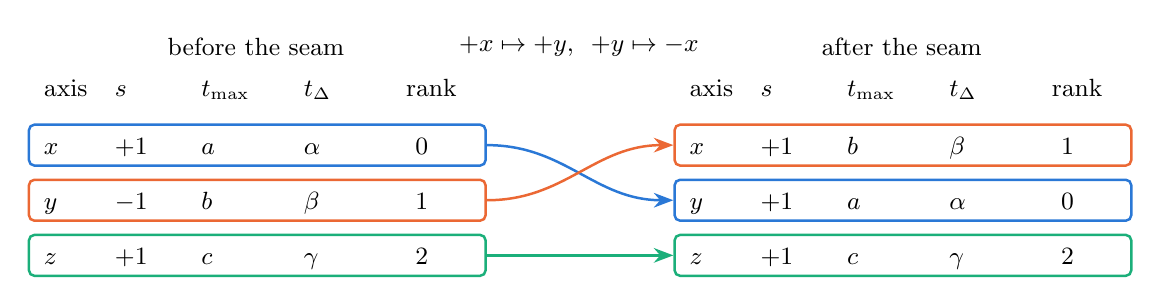
\begin{tikzpicture}[font=\small,
    row/.style={draw=#1, line width=0.9pt, rounded corners=2pt, minimum height=5.2mm,
                minimum width=58mm, inner sep=0pt},
    cell/.style={anchor=base west, inner sep=0pt}]
  \newcommand{\staterow}[8]{% x, y, colour, axis, step, tmax, tdelta, rank
    \node[row=#3, anchor=west] (#4) at (#1,#2) {};
    \node[cell] at ([xshift=2mm,yshift=-1.2mm]#4.west) {\makebox[9mm][l]{#5}\makebox[11mm][l]{#6}\makebox[13mm][l]{#7}\makebox[13mm][l]{#8}};
  }
  \node[cell] at (0.2,0.62) {\makebox[9mm][l]{axis}\makebox[11mm][l]{$s$}\makebox[13mm][l]{$\tmax$}\makebox[13mm][l]{$\tdelta$}\makebox[10mm][l]{rank}};
  \node[cell] at (8.4,0.62) {\makebox[9mm][l]{axis}\makebox[11mm][l]{$s$}\makebox[13mm][l]{$\tmax$}\makebox[13mm][l]{$\tdelta$}\makebox[10mm][l]{rank}};
  \staterow{0}{0}{s1}{bx}{$x$}{$+1$}{$a$}{$\alpha$}
  \staterow{0}{-0.7}{s2}{by}{$y$}{$-1$}{$b$}{$\beta$}
  \staterow{0}{-1.4}{s3}{bz}{$z$}{$+1$}{$c$}{$\gamma$}
  \staterow{8.2}{0}{s2}{ax}{$x$}{$+1$}{$b$}{$\beta$}
  \staterow{8.2}{-0.7}{s1}{ay}{$y$}{$+1$}{$a$}{$\alpha$}
  \staterow{8.2}{-1.4}{s3}{az}{$z$}{$+1$}{$c$}{$\gamma$}
  \node[anchor=base west] at ([xshift=48mm,yshift=-1.2mm]bx.west) {0};
  \node[anchor=base west] at ([xshift=48mm,yshift=-1.2mm]by.west) {1};
  \node[anchor=base west] at ([xshift=48mm,yshift=-1.2mm]bz.west) {2};
  \node[anchor=base west] at ([xshift=48mm,yshift=-1.2mm]ax.west) {1};
  \node[anchor=base west] at ([xshift=48mm,yshift=-1.2mm]ay.west) {0};
  \node[anchor=base west] at ([xshift=48mm,yshift=-1.2mm]az.west) {2};
  \draw[s1, line width=0.9pt, -{Stealth}] (bx.east) .. controls +(1,0) and +(-1,0) .. (ay.west);
  \draw[s2, line width=0.9pt, -{Stealth}] (by.east) .. controls +(1,0) and +(-1,0) .. (ax.west);
  \draw[s3, line width=0.9pt, -{Stealth}] (bz.east) -- (az.west);
  \node at (2.9,1.25) {before the seam};
  \node at (11.1,1.25) {after the seam};
  \node at (7.0,1.25) {$+x \mapsto +y$, \ $+y \mapsto -x$};
\end{tikzpicture}
\caption{The stepping state of a ray before and after a seam that turns a quarter about $z$.
Each row moves to the axis the turn sends its axis to, the step of the old $y$ axis changes
sign, and no value is recalculated. The rank of a row is the axis it had in the frame the ray
started in (\cref{sec:traversal}).}
\label{fig:state}
\end{figure}

\paragraph{Ties.} A ray through a voxel edge reaches two faces at the same distance, and the
order in which it crosses them decides which voxel it visits. A traversal usually breaks such a
tie by axis number. A seam renumbers the axes, and a ray that crossed one would then visit a
different voxel from its uncut trace; a test of rays sent from voxel centres along the 26 lattice
directions found one that visited 9 voxels where its uncut trace visited 10. The cursor
therefore carries a fourth per-axis value, the \emph{rank}: the number the axis had in the frame
the ray started in. Ties go to the larger rank, and the rank is permuted with the rest of the
state.

\paragraph{Counted steps.} The usual update $\tmax[i] \leftarrow \tmax[i] + \tdelta[i]$ rounds at
every step, and while $\tmax$ stays within one binade the rounding of a fixed addend has a constant
bias. The cursor instead stores the distance $f_i$ to the first face and the number $k_i$ of faces
crossed, and computes $\tmax[i] = f_i + k_i\,\tdelta[i]$ at each step, which rounds twice whatever the
length of the ray. Both $f$ and $k$ are per-axis values and are permuted at a seam.
\Cref{sec:measurements} reports the two forms side by side.

\begin{proposition}
\label{prop:agreement}
Let the map of every seam of a world be $c \mapsto Rc + o$ with $R$ a signed permutation matrix
and $o$ an integer vector. Let a ray be given by an origin, a direction and a starting voxel in
one room, and let its uncut trace be computed in the frame of that room by the same stepping
rule, with ties broken by axis number, the larger number first, and with no step taken to a face
at infinite distance. Then the cursor above takes the same number of steps as the uncut trace, at each step it
reports the same single-precision distance, and after each step it is in the voxel that the
composition of the maps of the seams crossed so far assigns to the voxel of the uncut trace.
\end{proposition}

\begin{proof}
Let $\pi$ be the permutation from the axes of the starting frame to the axes of the current
frame, composed from the turns of the seams crossed so far. We show by induction on the number
of steps that, for each starting axis $i$, the cursor's $\tmax$, $\tdelta$, $f$ and $k$ on axis
$\pi(i)$ are the uncut trace's on axis $i$, as the same floating-point numbers, and that the
cursor's rank on axis $\pi(i)$ is $i$. Both traces initialise the state from the same origin,
direction and voxel by the same operations, with $\pi$ the identity, which gives the base case.
For the step, the cursor chooses the least axis under the order ``smaller $\tmax$ first, and
among equal $\tmax$ the larger rank first''. The ranks are distinct and $\tmax$ is never a NaN,
because $\tdelta$ is never negative and never a NaN and the initial $\tmax$ is clamped at zero by an
operation that discards a NaN; the order is therefore total, and it reads only the pairs
$(\tmax, \text{rank})$. By the induction hypothesis these are the uncut trace's pairs
$(\tmax[i], i)$, and the uncut trace orders its axes by the same rule. If the uncut trace
chooses $i$, the cursor chooses $\pi(i)$, and both report the same $\tmax$. Both then
increment $k$ and evaluate $f + k\,\tdelta$ on equal operands, with equal results. If the face
lies on a seam, the cursor copies the four values of each axis to the axis the turn sends it to,
which restores the hypothesis for $\pi$ followed by the turn. The voxel is updated by a unit
step or by an integer map, and both are exact. Since the two traces visit corresponding voxels
at equal distances, they read the same materials and stop at the same step.
\end{proof}

The proof uses two hypotheses, and each is needed. A turn that is not a signed permutation mixes
the axes, the per-axis values cannot then be moved, and the state must be recomputed, as in every
method of \cref{sec:related} that admits a general matrix. The rank is needed because the tie
order otherwise depends on the frame, and the ray of the previous paragraph is a counterexample. The proposition does not cover
the hit point: the cursor also carries the ray's origin into each new frame for callers that
want it, by floating-point arithmetic that the traversal never reads.

\section{One adjacency for every subsystem}
\label{sec:subsystems}

Everything in the engine that moves does so by crossing faces, through one function that
returns the voxel beyond a face and the seam crossed to reach it.

\paragraph{Light.} Lamp light and sky light are flooded breadth first from their sources, losing
one level per voxel, as in block-based games. The flood steps through that function, and light
therefore crosses seams of any turn with no code of its own. A lamp lights the room beyond a
doorway, and in a room glued to itself one lamp lights every copy.

\paragraph{Sprites.} A moving figure is a small block of voxels placed into a per-frame overlay
by walking the lattice from its anchor voxel. A figure that stands in a doorway has its front
half in the next room, turned as the seam turns it, and a ray is traced against the world and
the overlay together.

\paragraph{Bodies.} A walking body is a box with a frame, an orientation that takes the body's
axes to the room's. When the body's middle crosses a seam, its position goes through the seam's
map and its frame is composed with the seam's turn. Gravity acts along the body's own down
axis, and ``down'' is consequently whatever the path that brought the body here says it is. A
world can overrule the path: a room may declare which way is up, and a body that arrives turned
is then stood upright, as Prey does at its portals~\cite{prey}.

\paragraph{Rendering.} The renderer traces one primary ray per sample and one shadow ray per lit
hit through the same cursor, and reads ambient occlusion and flooded light from the voxels
around the hit, found by lattice walks when the hit is next to a seam.

\section{The test: cut, turn and re-glue}
\label{sec:test}

We specify the engine by a single property, which we test by building a random world twice: once
whole, as a box of $2n \times n \times n$ voxels, and once cut into two cubes, with the second cube turned by
an orientation $R$ and glued back to the first along the cut. The two worlds are the same space
in different coordinates, and no observable may differ between them. The test runs for all 48
orientations and for each kind of thing that moves (\cref{tab:tests}). Changing the frame of a
region and compensating on its boundary is a gauge transformation, and lattice QCD codes test
their observables under it~\cite{chroma}; as a testing technique this is a metamorphic
relation~\cite{chen1998}, of the kind GraphicsFuzz applies to shader
compilers~\cite{donaldson2017}.

\begin{table}[t]
\centering
\small
\begin{tabular}{@{}lp{0.42\linewidth}p{0.33\linewidth}@{}}
\toprule
Subject & Per orientation & Must equal the whole world's \\
\midrule
Rays & 400 random rays, and rays from voxel centres along the 26 lattice directions & hit, voxel, face, material, step count; distance bit for bit \\
Poses & a point moved 60 times across the cut & voxel and frame; position to 0.002 \\
Light & a world with 35\% solid voxels and two lamps in one half & lamp and sky level of every voxel \\
Sprites & an asymmetric sprite placed four times near the cut, then 200 rays, each traced again looking past one sprite as its viewer would & occupied voxels; ray results bit for bit \\
Bodies & a 3\,s walk over a step, round a post and through a turn & room, frame, grounded state; position to 0.002 \\
Frames & one $96 \times 54$ picture taken from the uncut half & every pixel \\
\bottomrule
\end{tabular}
\caption{The cut, turn and re-glue test, which runs for each of the 48 orientations. In the frame
test no pixel of the 248{,}832 differed by one grey level. Each row was also checked to fail
when its subject is broken: light that ignores seams, a sprite, a body or a sun direction that is
not turned.}
\label{tab:tests}
\end{table}

A world with one cut tests the rule for ties across one seam only, and a comparison of final
hits rarely detects a wrong order of two tied faces. A second ray test therefore cuts a cube of
15 voxels a side into 125
blocks, turns each block by a random orientation, and compares the two cursors after every face
they cross: distance, voxel, entry face and material, for random rays and for rays along lattice
directions with unequal components, which cross up to a dozen seams. With ties broken by the
current axis number, this test and the lattice-direction rays of \cref{tab:tests} fail, and the
measurement of \cref{sec:measurements}, which compares final hits, still finds agreement on
219{,}998 of 220{,}000 rays.

The sprite rays of \cref{tab:tests} include rays that look past the voxels of one figure near
their start, as a renderer does so that a viewer does not see the inside of its own figure. The
rule for this reads the distance travelled and not the number of seams crossed: that number
differs between the cut world and the whole one, and under a rule that reads it a viewer
standing across a seam sees its own voxels on the far side, which the test rejects.

\section{Measurements}
\label{sec:measurements}

\paragraph{Setup.} The test of \cref{sec:test} crosses one seam, and to cross many we use the
quarter-turn space of Conway and Rossetti~\cite{conway2003} with a voxel lattice in it: a cube of
8 voxels a side whose $x$ and $y$ faces are glued to their opposites by translations and whose
$z$ faces are glued with a quarter turn, with 15\% of its voxels solid, in which a ray never
leaves. Each ray passes its first $c$ seams unobstructed and then stops at the first solid voxel, for 11
values of $c$ from 0 to 1{,}000 and 20{,}000 uniformly random rays per value. The same ray is
traced in the unrolled space twice: in single precision, which is the uncut trace, and in double
precision, which we take as the true ray. A voxel of the unrolled space is looked up by folding
its integer coordinates into the cube, and a test checks the folding against the engine's lattice
walk. The numbers below are from a run whose seeds differ from those the experiment was designed
on; the two runs agree in every qualitative statement made here.

We compare six ways of crossing: \emph{permute, counted steps}, which is the engine's cursor,
\emph{permute, running total}, which is the same rule with the usual update of $\tmax$, and
four baselines. \emph{Recompute at the crossing point} transforms the crossing point and direction, carries the
voxel through the integer map, restarts the distance and recomputes the state; boxspace works
this way in every cube~\cite{boxspace}. \emph{Recompute from the origin} transforms the origin
and direction, keeps one running distance, takes the voxel as the truncated point at that
distance and resets the state, as fishpye does~\cite{fishpye}. \emph{Nudge and floor} moves the
crossing point a distance $\varepsilon$ along the ray and takes the voxel as the floor of the
transformed point, which is the rule noeuclid applies at every voxel with
$\varepsilon = 0.01$~\cite{noeuclid}. \emph{Matrix per cell} keeps no stepping state: the ray is
a position and a tangent in the coordinates of the cell it is in. In every cell the distance to
each of the six walls is computed, the position is moved to the nearest wall, and a matrix takes
the position and the tangent into the coordinates of the next cell, whether or not the wall is a
seam. This is the Euclidean branch of HyperRogue's ray shader, with its expressions in its
order, and the distance is the shader's sum of the wall-to-wall
distances~\cite{hyperroguesrc}. The shader declares its numbers \texttt{mediump}, to which
desktop OpenGL gives 32 bits, and we run it in single precision. The four baselines are our
re-implementations in this world, written from the cited sources, and are not the original
programs. Where the fishpye
rule puts a point outside the room we move it to the nearest voxel inside, which favours the
rule.

\begin{table}[t]
\centering
\small
\begin{tabular}{@{}lrrrr@{}}
\toprule
Seams crossed & 1 & 10 & 100 & 1{,}000 \\
\midrule
\tablebody tables/agreement.tex
\bottomrule
\end{tabular}
\caption{Rays, of 20{,}000, whose result equals the uncut trace in voxel, face, material, step
count and distance, the distance compared bit for bit. The two permuting methods are each
compared with the uncut trace in their own form of stepping state, and the other methods with
the uncut trace in counted steps.}
\label{tab:agreement}
\end{table}

\paragraph{Agreement.} Both permuting methods equal their uncut traces on all 20{,}000 rays at
each of the 11 crossing counts (\cref{tab:agreement}), which is \cref{prop:agreement} observed
on 220{,}000 rays. No baseline does: at 1{,}000 crossings recomputation from the origin agrees
on 8{,}980 rays, recomputation at the crossing point on 792 and the matrix per cell on 197. The
matrix per cell is not a traversal of the same form, and its distances differ from the uncut
trace's in the last bits on 10{,}866 of 20{,}000 rays that cross no seam.

\begin{table}[t]
\centering
\small
\setlength{\tabcolsep}{4pt}
\begin{tabular}{@{}lrlrlrlrl@{}}
\toprule
Seams crossed & \multicolumn{2}{c}{1} & \multicolumn{2}{c}{10} & \multicolumn{2}{c}{100} & \multicolumn{2}{c}{1{,}000} \\
\tablebody tables/distance.tex
\midrule
& off & error & off & error & off & error & off & error \\
\midrule
\tablebody tables/accuracy.tex
\bottomrule
\end{tabular}
\caption{Accuracy against the true ray. ``Off'' is the number of rays, of 20{,}000, that end on a
voxel or face other than the true ray's. ``Error'' is the median distance error, in voxels, of
the rays that end on the true surface.}
\label{tab:accuracy}
\end{table}

\begin{figure}[t]
\centering
\begin{tikzpicture}
\begin{loglogaxis}[
    width=0.74\linewidth, height=6.4cm,
    xlabel={seams crossed before the hit}, ylabel={median distance error (voxels)},
    xmin=1, xmax=1000, ymin=1e-7, ymax=1,
    grid=major, grid style={gray!25},
    legend pos=north west, legend cell align=left, legend style={font=\footnotesize, draw=none},
    tick label style={font=\footnotesize}, label style={font=\small}]
  \addplot[s1, line width=1pt, mark=*, mark size=1.6pt] table[x=crossings, y=median] {figures/data/engine.dat};
  \addlegendentry{permute, counted steps (ours)}
  \addplot[s2, line width=1pt, mark=square*, mark size=1.6pt] table[x=crossings, y=median] {figures/data/perm-run.dat};
  \addlegendentry{permute, running total}
  \addplot[s3, line width=1pt, dashed, mark=triangle*, mark size=2pt] table[x=crossings, y=median] {figures/data/recompute.dat};
  \addlegendentry{recompute at the crossing point}
  \addplot[s4, line width=1pt, densely dotted, mark=diamond*, mark size=2pt] table[x=crossings, y=median] {figures/data/fishpye.dat};
  \addlegendentry{recompute from the origin (fishpye)}
  \addplot[s5, line width=1pt, dashdotted, mark=pentagon*, mark size=2pt] table[x=crossings, y=median] {figures/data/cell-matrix.dat};
  \addlegendentry{matrix per cell (HyperRogue)}
\end{loglogaxis}
\end{tikzpicture}
\caption{Median distance error against the number of seams crossed, for the rays that end on the
true surface. One thousand crossings is a mean distance of 5{,}396 voxels. Numbers are in
\cref{tab:accuracy}.}
\label{fig:error}
\end{figure}

\paragraph{Accuracy.} Agreement with the uncut trace says nothing about the error of the uncut
trace. With a running total the error grows with the square of the distance
(\cref{fig:error}): at 1{,}000 crossings, a mean distance of 5{,}396 voxels, the median error is
$8.7\times10^{-2}$ voxels and 2{,}890 of 20{,}000 rays end on another surface
(\cref{tab:accuracy}). Seams play no part in this error, since the uncut trace with a running
total has it bit for bit. The recomputing methods work their distances out again at each seam
and do not accumulate it, and a permuting traversal with a running total is the least accurate
method in the table on long rays. With counted steps the median error at 1{,}000
crossings is $1.7\times10^{-4}$ voxels and 7 rays are off, against $2.4\times10^{-4}$ and 12 for
recomputation from the origin and $4.2\times10^{-3}$ and 1 for recomputation at the crossing
point. Up to 200 crossings the engine and the two recomputing methods each put at most one ray in
20{,}000 on another surface. The matrix per cell maintains its position within one voxel of the
origin of its coordinates, and it finds the surface as reliably as any method in the table: no
ray is off up to 200 crossings and 4 are off at 1{,}000. Its distance, which HyperRogue uses for fog only, is a sum and drifts as the running total does,
to a median error of $2.9\times10^{-2}$ voxels at 1{,}000 crossings. Nudge and floor is off for 47 to 74 rays in 20{,}000 with
$\varepsilon = 10^{-2}$ and for 4 to 9 with $\varepsilon = 10^{-3}$, at every crossing count from
1 to 1{,}000, because the nudge carries a ray that crosses near a voxel edge into the
neighbouring voxel.

\begin{table}[t]
\centering
\small
\begin{tabular}{@{}lrr@{}}
\toprule
& Plain step (ns) & Extra per crossing (ns) \\
\midrule
\tablebody tables/cost.tex
\bottomrule
\end{tabular}
\caption{Cost of a step and of a crossing, fitted by least squares to the time per step in empty
quarter-turn spaces of side 4, 8, 16, 32 and 64, in which a fraction $1/\text{side}$ of the steps
are crossings. One thread of an Apple M3; each time is the fastest of nine repeats of 4{,}000
rays of 1{,}000 steps. The first row is the engine's cursor; the others are loops written against
its public API.}
\label{tab:cost}
\end{table}

\paragraph{Cost.} A crossing by permutation costs 25\,ns more than a plain step and a crossing
by recomputation 41 to 43\,ns (\cref{tab:cost}); the difference is three divisions and the
transformation of a point. Counted steps cost 0.7\,ns more per plain step than a running total
when the two forms are measured in the same loop (7.5 against 6.7\,ns). Crossing costs varied by
up to 5\,ns between runs. The matrix per cell is a method for a GPU shader and is not timed.

\begin{table}[t]
\centering
\small
\begin{tabular}{@{}lrr@{}}
\toprule
& Fastest (ns) & Median (ns) \\
\midrule
\tablebody tables/linktest.tex
\bottomrule
\end{tabular}
\caption{Time per step in a room of side 128 with no seams: 40{,}000 rays from its middle, 4.7
million steps, 31 repeats of each loop in turn, one thread of an Apple M3.}
\label{tab:linktest}
\end{table}

\paragraph{Overhead.} A world with no seams still tests one bit at each face. We copied the
cursor's loop over an array of the engine's 16-bit cells and timed it with that test compiled in
and with it left out (\cref{tab:linktest}). The test costs 0.16\,ns of a 4.83\,ns step by the
fastest repeats and 0.15\,ns by the medians, which is 3\%, and between 0.08 and 0.16\,ns in
five other runs. The engine's cursor takes
7.59\,ns for the same step. The 2.8\,ns it adds to the copied loop are not the link test: the
cursor finds its room by index at each step, returns the face and the seam it crossed, and is
called across a crate boundary, and we have not separated these costs.

\begin{table}[t]
\centering
\small
\begin{tabular}{@{}lrrr@{}}
\toprule
& Pixels that differ & On another surface & Most in one view \\
\midrule
\tablebody tables/pixels.tex
\bottomrule
\end{tabular}
\caption{Pixels, of 1{,}843{,}200 in 8 views, whose 8-bit colour is not that of the picture the
uncut trace draws. ``On another surface'' counts those whose ray stops on another voxel or face;
the rest stop on the same surface at a distance that rounds to another colour. A view has
230{,}400 pixels.}
\label{tab:pixels}
\end{table}

\begin{figure}[tb]
\centering
\setlength{\tabcolsep}{2pt}
\begin{tabular}{@{}cc@{}}
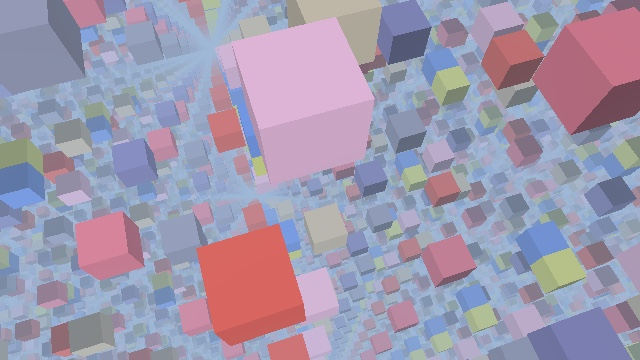
\includegraphics[width=0.495\linewidth]{figures/pixels_uncut.jpg} &
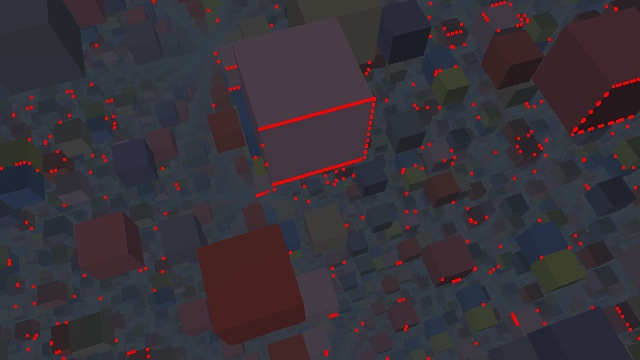
\includegraphics[width=0.495\linewidth]{figures/pixels_marked.jpg}
\end{tabular}
\caption{One of the 8 views of \cref{tab:pixels}. Left: the quarter-turn space of side 8 with
2\% of its voxels solid, drawn by the uncut trace. Right: the same picture dimmed, with the
pixels at which nudge and floor with $\varepsilon = 10^{-2}$ differs from it in red, each mark
enlarged to 3 by 3 pixels.}
\label{fig:pixels}
\end{figure}

\paragraph{Pictures.} We drew 8 views of $640\times360$ pixels in the same space with 2\% of
its voxels solid, one ray a pixel, from random positions and in random directions
(\cref{fig:pixels}). A ray crosses 8.0 seams on average and at most 502. The colour of a pixel
is a function of the material and the face the ray stops on, faded with distance and rounded to
8 bits a channel; the shading reads no hit point and casts no shadow rays. Each method's
pictures are compared with those its uncut trace draws (\cref{tab:pixels}). The two permuting
methods differ in no pixel, and the two recomputing methods and the matrix per cell in 6 to 23
pixels, at most one in 80{,}000, although 43 to 67\% of their rays differ from the uncut trace
in some bit. Nudge and floor differs in 254 pixels with $\varepsilon = 10^{-3}$ and in
2{,}279 with $\varepsilon = 10^{-2}$, up to 430 in one view, and 2{,}241 of the 2{,}279 are on
another voxel or face: single pixels along voxel edges.

\section{Worlds}
\label{sec:worlds}

\begin{figure}[t]
\centering
\setlength{\tabcolsep}{2pt}
\begin{tabular}{@{}cc@{}}
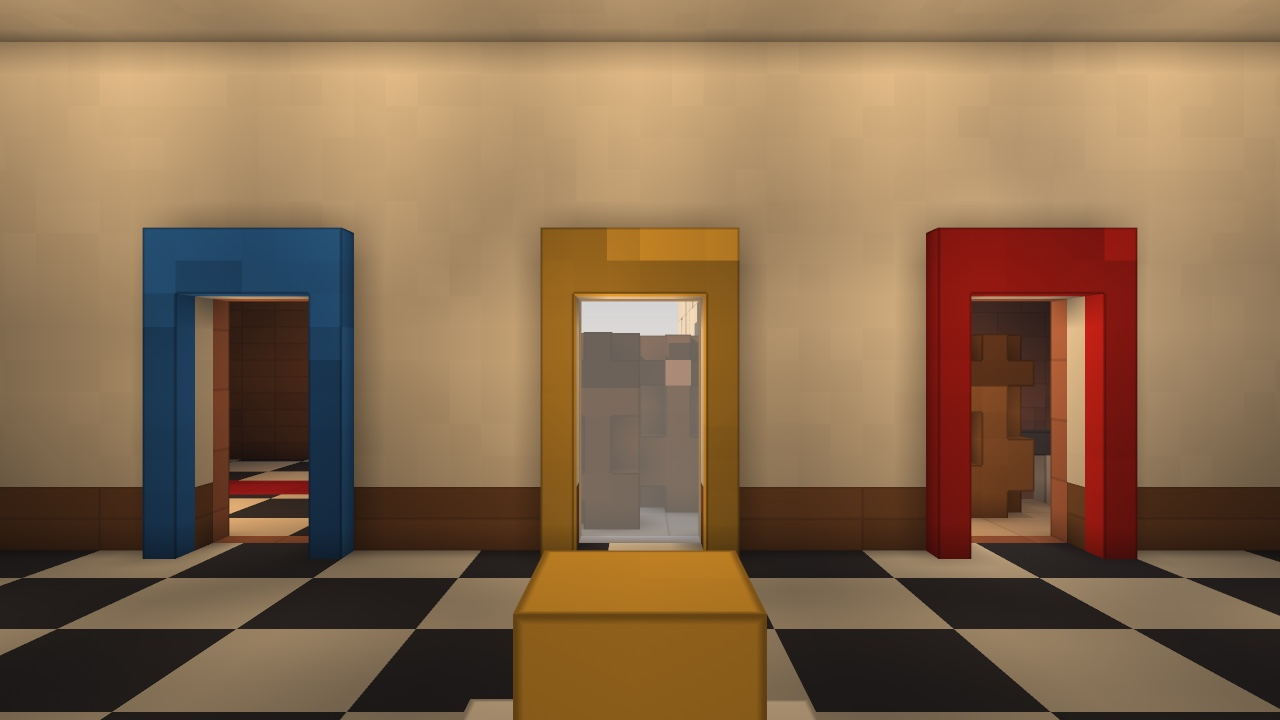
\includegraphics[width=0.495\linewidth]{figures/gallery.jpg} &
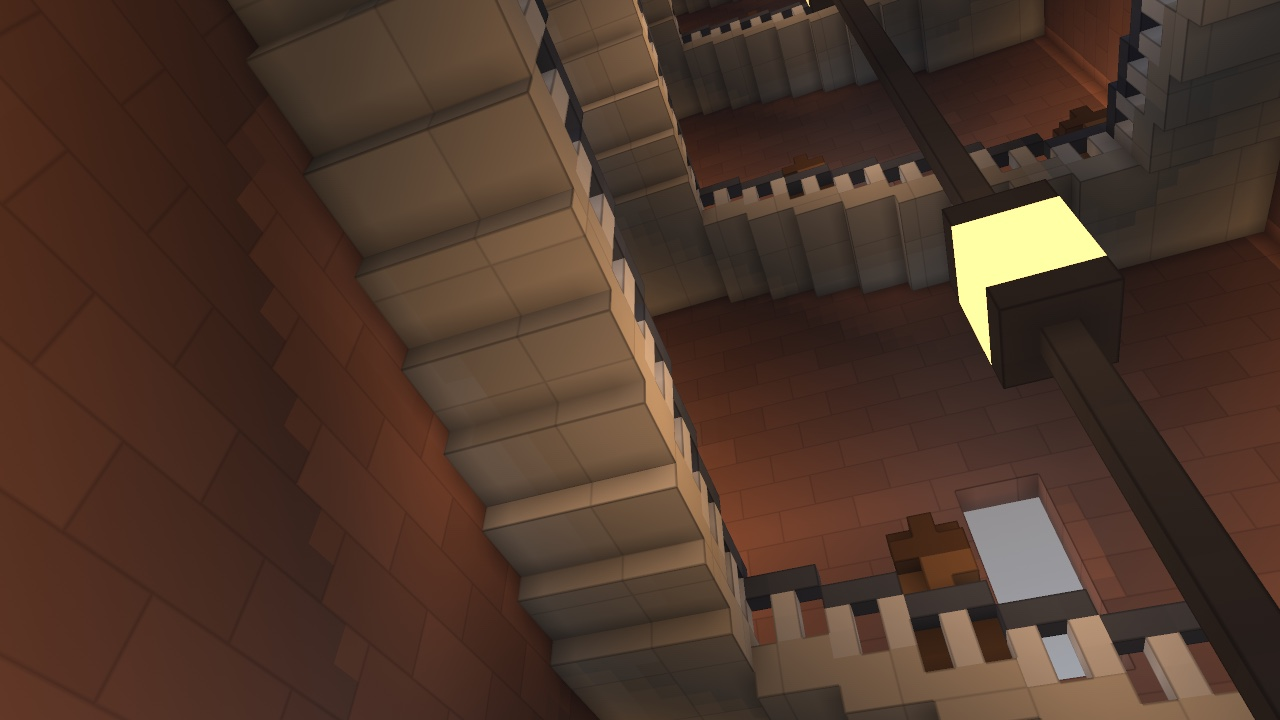
\includegraphics[width=0.495\linewidth]{figures/well.jpg} \\
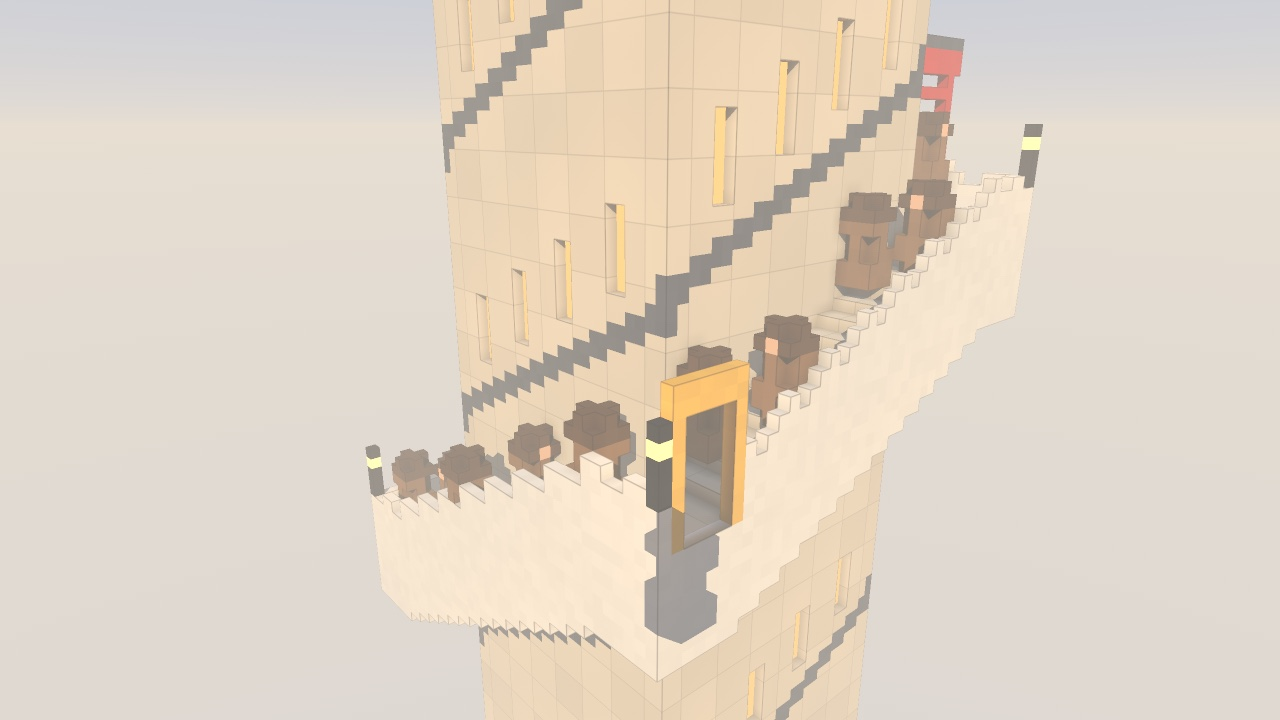
\includegraphics[width=0.495\linewidth]{figures/tower.jpg} &
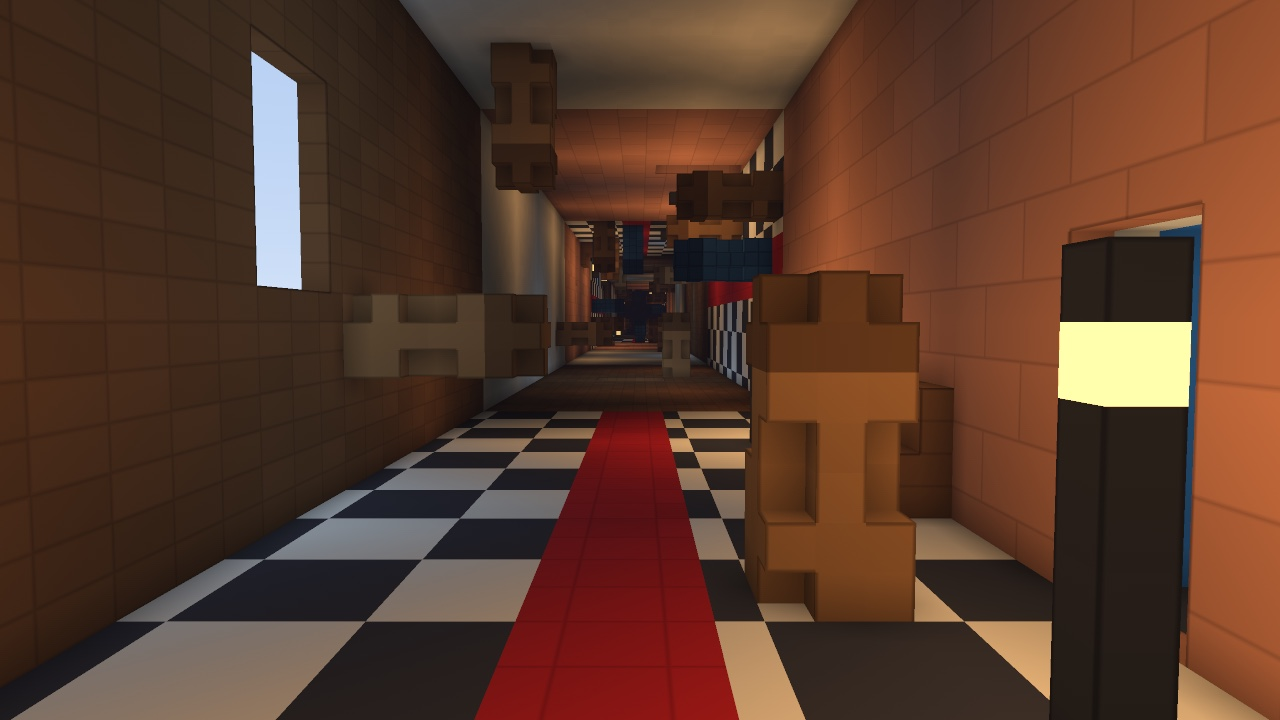
\includegraphics[width=0.495\linewidth]{figures/hall.jpg}
\end{tabular}
\caption{The four worlds, rendered by the engine. Top: the Gallery, with a door onto each of
the other worlds, and the Well, looking up its shaft. Bottom: the Tower, whose walkway descends
all the way round, and the Hall, in which the walkers on the walls and the ceiling are the
walkers on the floor seen through the seam.}
\label{fig:worlds}
\end{figure}

The engine ships four worlds (\cref{fig:worlds}), each built from the operations of \cref{sec:model}. The
\emph{Gallery} is an ordinary room with three doors, each glued to a door of another world, and
a mirror, which is a seam from a rectangle of faces to itself with a reflection. The \emph{Well}
is a square stairwell 32 voxels tall whose top face is glued to its bottom face; one lap down the
stairs returns a walker to the landing it left. The \emph{Hall} is a corridor of $22 \times 22$
voxels in section and 56 long whose far end is glued to its near end with a quarter turn about
its axis. It is a piece of the quarter-turn space: a body that walks its length stands on what
was the wall, and after four lengths it is upright where it began.

The \emph{Tower} is a walkway round the outside of a tower that descends on all four sides and
closes. East of the tower, space is cut along a half-plane and glued back 60 voxels out of step
along the vertical axis, and the walkway's lowest step meets its highest across the cut. This is
Volterra's cut-and-reglue construction of a dislocation~\cite{volterra1907,kleman2008}: the cut
is the cut surface, its inner edge, which runs up the east wall of the tower, is the dislocation
line (\cref{fig:tower}), and a lap of the walkway is a Burgers circuit whose closure failure, 60 voxels parallel to the
line, is the Burgers vector of a screw dislocation. In the convention of Hirth and
Lothe~\cite[p.~22]{hirth1968}, with the sense $\xi$ of the line taken upward, a circuit that is
right-handed about $\xi$ and closes in the perfect lattice finishes 60 voxels below its start in
the glued one, which gives $b \cdot \xi = -60$: a left-handed screw dislocation whose Burgers
vector is a lattice vector. A test in the repository walks this circuit through the engine's
lattice walk. The walkway rises counterclockwise seen from above, as a right-handed stair does,
and the left-handed helicoid of the lattice planes round the line is what closes it. The
identification of the Penrose staircase~\cite{penrose1958} with a screw dislocation follows from these
definitions.

\begin{figure}[t]
\centering
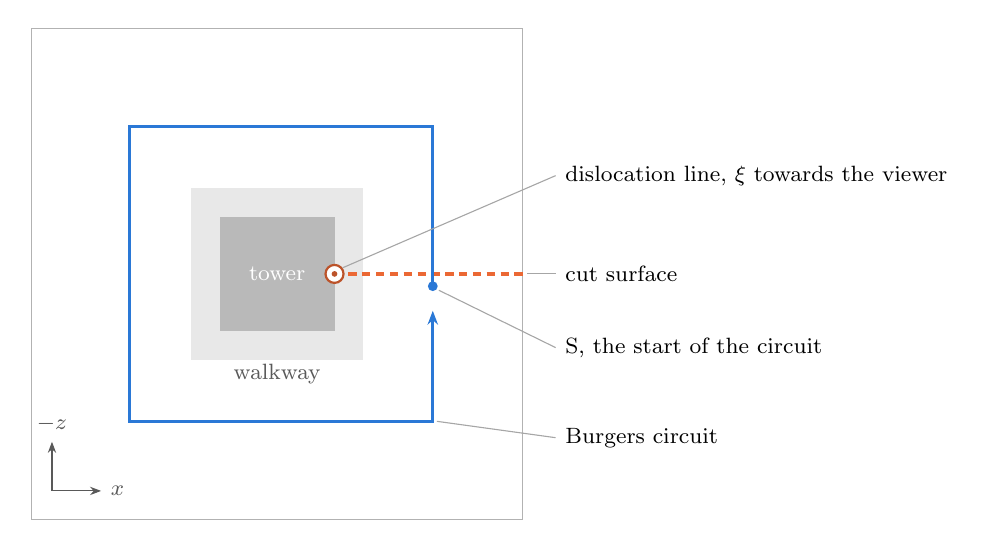
\begin{tikzpicture}[x=0.052cm, y=-0.052cm, font=\footnotesize]
  % Plan of the Tower's room seen from above: x to the right, z down the page.
  \draw[gray!60] (0,0) rectangle (120,120);
  \fill[gray!18] (39,39) rectangle (81,81);
  \fill[gray!55] (46,46) rectangle (74,74);
  \node[white] at (60,60) {tower};
  \node[gray!70!black] at (60,84.5) {walkway};
  % The cut, edge on, from the tower's east wall to the edge of the room.
  \draw[s2, line width=1.2pt, dash pattern=on 3pt off 2pt] (74,60) -- (120,60);
  % The Burgers circuit: right-handed about xi, which is counterclockwise from above.
  \draw[s1, line width=1pt, -{Stealth[length=5pt]}] (98,63) -- (98,24) -- (24,24) -- (24,96) -- (98,96) -- (98,69);
  \fill[s1] (98,63) circle (1.2);
  % The dislocation line, seen end on, with its sense towards the viewer.
  \draw[s2!80!black, fill=white, line width=0.8pt] (74,60) circle (2.2);
  \fill[s2!80!black] (74,60) circle (0.7);
  % Labels, in a column to the right of the room.
  \node[anchor=west] (line) at (128,36) {dislocation line, $\xi$ towards the viewer};
  \node[anchor=west] (cut) at (128,60) {cut surface};
  \node[anchor=west] (start) at (128,78) {S, the start of the circuit};
  \node[anchor=west] (loop) at (128,100) {Burgers circuit};
  \draw[gray!70, thin] (line.west) -- (76,58.5);
  \draw[gray!70, thin] (cut.west) -- (121,60);
  \draw[gray!70, thin] (start.west) -- (99.5,64);
  \draw[gray!70, thin] (loop.west) -- (99,96);
  % Axes.
  \draw[-{Stealth[length=4pt]}, gray!70!black] (5,113) -- (17,113) node[right] {$x$};
  \draw[-{Stealth[length=4pt]}, gray!70!black] (5,113) -- (5,101) node[above] {$-z$};
\end{tikzpicture}
\caption{The Tower's room seen from above. The cut surface is a half-plane east of the tower,
across which space is glued 60 voxels out of step along the vertical axis. Its inner edge is the
dislocation line, whose sense $\xi$ we take upward, towards the viewer. The circuit is
right-handed about $\xi$ and closes in a perfect lattice; in the glued lattice it finishes 60
voxels below its start S.}
\label{fig:tower}
\end{figure}

\begin{table}[t]
\centering
\small
\begin{tabular}{@{}lrr@{}}
\toprule
View & One thread (ms) & Eight cores (ms) \\
\midrule
\tablebody tables/frames.tex
\bottomrule
\end{tabular}
\caption{Time to render one frame of $640 \times 360$ pixels with one sample a pixel, shadows,
ambient occlusion and outlines, on an Apple M3 (four performance and four efficiency cores). Each
time is the median of five runs. The views are those of \cref{fig:worlds}, and Mirror is the
Gallery's mirror.}
\label{tab:frames}
\end{table}

The renderer traces every pixel on the CPU with no acceleration structure, and a frame takes
27 to 80\,ms on eight cores (\cref{tab:frames}). The Tower is the slowest view because its room
is open air, which a ray crosses one voxel at a time.

\section{Related work}
\label{sec:related}

Rendering by walking a graph of cells through their openings goes back to Jones~\cite{jones1971}, as
described by Luebke and Georges~\cite{luebke1995}, who give each portal ``a polygonal boundary and
a pointer to the adjacent cell'' and, following Teller (1992), treat a mirror as a portal that
transforms the cell it is attached to. Descent~\cite{descent} made the adjacency of six-sided
segments the one structure that its renderer, collision, AI, weapons and static light all walk,
with every link the identity in one world frame. Dungeon Master~\cite{dungeonmaster} turned
everything that crossed a teleporter square by that square's rotation. Prey~\cite{prey} rotates a
body's axes by the portal map and then sets its gravity, and Immersive
Portals~\cite{immersiveportals} does the same with rotated portals, draws an entity that
straddles a portal on both sides, and builds a mirror as a portal whose destination is itself.
Per-face adjacency as the primitive, one traversal shared by every subsystem, frames turned by
links and mirrors as self-links are therefore all prior practice, and we claim none of them.

fishpye~\cite{fishpye} is a voxel ray tracer after Amanatides and Woo in which a portal is a
block type with a $4\times4$ matrix; at a portal it transforms the ray's origin and direction,
takes the voxel as the truncated point at the running distance, and resets the step, $\tdelta$
and $\tmax$. noeuclid~\cite{noeuclid} traces a 3D texture whose ``jump'' cells carry a
$3\times3$ matrix and an offset; it has no stepping state, moves the sample point 0.01 past each
voxel boundary, and takes the voxel as the floor of that point. boxspace~\cite{boxspace} is the
closest prior work: its world is a list of unit cubes, each face stores a target cube and one of
the 24 rotations of the cube, the integer cube index is carried through the link, and the exit
face is recomputed from the local position in every cube.
HyperRogue~\cite{hyperrogue2017} stores a neighbour, a spin and a mirror flag for each face of
each cell, has supported twisted quotients of the Euclidean cube tiling since April 2019 and the
quarter-turn space since March 2020 at the latest, and since October 2019 has a ray-based
renderer that multiplies the ray's position and direction by a connection matrix at each cell
wall~\cite{kopczynski2022,celinska2022}. voxeltorus~\cite{voxeltorus} stores six neighbour
indices for every voxel, with translations only, and Jacob's Matrix~\cite{jacobsmatrix} has the
same architecture as ours in two dimensions: rooms that are dense grids, joined square to square
by portals that turn by a quarter. A voxel world whose faces are glued by cube symmetries, with
rays carried across the gluings, existed before this work in each of these.

Berger, Laier and Velho~\cite{berger2015} trace interior views of flat and hyperbolic
3-manifolds and orbifolds in image space. Their space is a polyhedron with an involution on its
faces and an isometry $g_i$ for each face whose inverse belongs to the paired face, which is our
pair of seams for a general polyhedron, and a ray that reaches face $i$ at a point $x$ continues
as its image under $g_i$ from $g_i(x)$. They set aside a ray through two faces at once as an
event of probability zero; on a lattice it is the tie of \cref{sec:traversal}. Novello, da Silva and Velho~\cite{novello2020}
path-trace quotient spaces, including the flat 3-torus and a dodecahedron whose faces are
mirrors, and Coulon, Matsumoto, Segerman and Trettel~\cite{coulon2022} ray-march the eight
Thurston geometries and their quotients, teleporting a ray's position and tangent by a face
pairing when it leaves the fundamental domain. These methods apply a floating-point isometry at
each crossing, and Coulon et al.\ note the ``potential accumulation of errors'' that follows.
The spaces our worlds are built from were drawn before: Curved Spaces~\cite{curvedspaces}
renders the quarter-turn space of Conway and Rossetti~\cite{conway2003}, as does HyperRogue, and
a closed staircase that always descends was made walkable in Nil geometry by Kopczy\'nski in 2020.

A world of unit cubes glued along faces by isometries is a classical object, a cubed complex in
the sense of Gromov~\cite{gromov1987} and of Bridson and Haefliger~\cite{bridson1999}, and away
from the rims of its seams it carries a $(G, X)$-structure~\cite{thurston1997} whose group is
generated by the integer translations and the 48 signed permutation matrices. The loop that
detects the Tower's dislocation is the circuit of Burgers (1939) and Frank~\cite{frank1951}, in the convention of Hirth and
Lothe~\cite{hirth1968}. The map we
attach to a seam, a signed permutation with an integer offset whose reverse is its inverse, is the
1-to-1 interface transform of the CGNS standard for multiblock grids~\cite{cgns} and the
transition function of hexahedral meshing~\cite{nieser2011,lyon2016}, where an edge whose
composed transition is not the identity is called singular. Ptex~\cite{burley2008} stores
per-face adjacency for textures and rotates its filter kernel when it crosses an edge.

Three things did not turn up in searches of engine and game source code, project pages, the
literature, GitHub code search, Shadertoy and two Reddit forums on 23 and 24 November 2026. The
first is a traversal that carries its Amanatides--Woo state across a gluing by permuting it:
fishpye resets the state, boxspace and noeuclid keep none, HyperRogue and the manifold ray
tracers transform the ray by a matrix, and the three grid raycasters with turned portals that
the code search found each cast a new ray at the portal~\cite{portalraycaster,ultimateraycasting,weblabyrinth}. The second is flood-filled voxel light that crosses
rotated gluings. The third is the test of \cref{sec:test} as the specification of an engine.

\section{Conclusion}

Restricting the gluings of a voxel world to the 48 symmetries of the cube lets a ray cross one
by permuting its stepping state, and the resulting trace is the uncut trace, which makes an
engine without seams an exact oracle for an engine with them. The same restriction lets light,
sprites and bodies use one adjacency, and one test cover all of them. The traversal needed
counted steps before it was also as accurate as recomputation on long rays.

A seam whose rim is exposed tears the picture, and the first piece of further work is a lint
that walks a Burgers circuit round every rim edge and reports the tear before a user sees it.
The second is storage: rooms are dense arrays, and chunks with a clearance field would let a ray
skip empty space without leaving the lattice a seam is defined on. The third is a GPU cursor,
since the cursor's loop fits a compute shader in which a seam is a table lookup.

\section*{Reproducibility}

The engine, the tests and the measurement programs are at
\url{https://github.com/no-way-labs/groxel}. \code{cargo test --workspace} runs the tests of
\cref{sec:test}, and \code{sh experiments/run.sh} regenerates every table and the data of
\cref{fig:error}, recording the machine, compiler and commit. The measurements here were made on
an Apple M3 with rustc 1.99.0 in release mode on one thread, and the workspace has no
dependencies outside itself.

\bibliographystyle{plain}
\bibliography{refs}

\end{document}
